
%----------------------------------------------------------------------------
\chapter{Overview of the approach}
%----------------------------------------------------------------------------

%%
%% Futásidejű dolgok és kódgenerálás is!
%%

In this chapter, the approach to monitoring of cyber-physical systems is presented, used by the developed framework. 
The architecture of the framework is depicted on figure~\ref{fig:approach}. 
The framework has a design-time and runtime part.
The design time part consists of the process of creating the artifacts, mainly program sources which will be responsible for runtime verification.

\begin{figure}[h]
	\begin{center}
		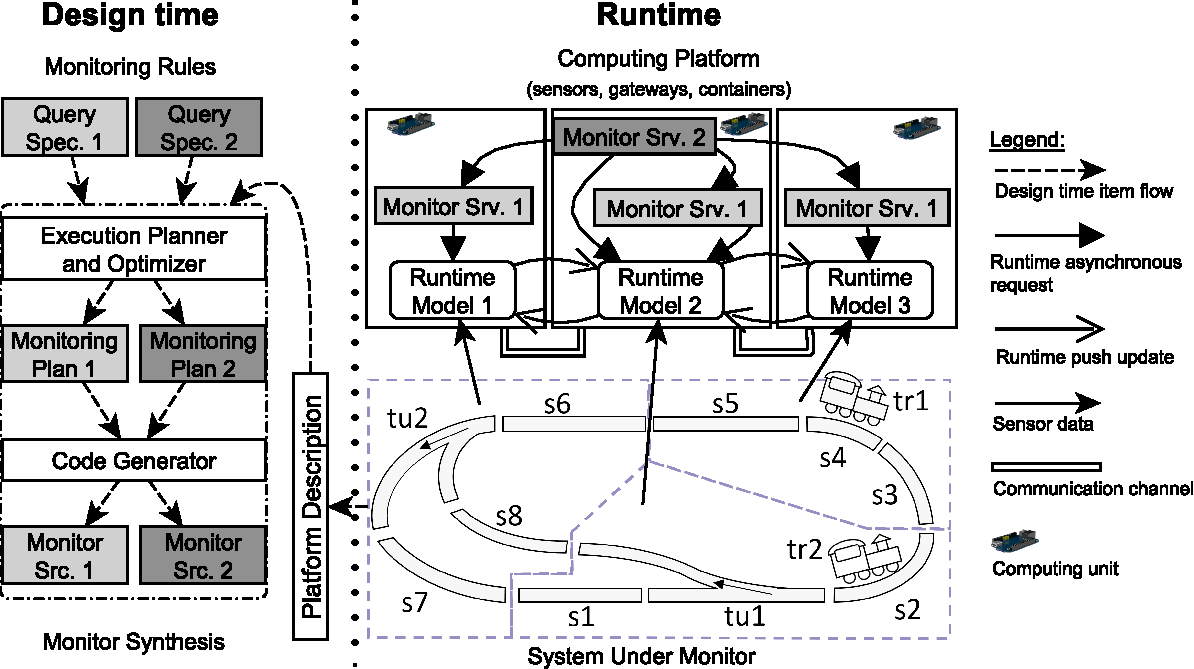
\includegraphics[width=\textwidth]{figures/fase-overview-crop.pdf}
		\caption{Approach for cyber-physical systems monitoring used by the presented framework }
		\label{fig:approach}
	\end{center}
\end{figure}

\section{Design time}

At first, the developer of the cps must design the models based on the structure of the target system using EMF Ecore modeling. 
The meta model of the living model defines the types of the graph elements, the possible edges between instances of given types, and attributes of instances of a given type. 
We generate \cpp{} source code from these models, that can be used to build up and update the living model of the system.

Then monitoring goals are defined as graph patterns. 
As patterns can refer to the meta model, it is a prerequisite for pattern definition. 
For graph pattern definition, the query language of \viatra{} is used (Viatra Query Language). 
From these patterns we create monitoring plans (local search plans). 
We use these plans to generate the source code of the monitoring components.

\section{Runtime}

At runtime, we rely on the generated monitor code and the generated classes. 
By instancing the classes, we create the nodes of the living model, create the references/edges between them and give the values of the attributes of the objects. 
With the physical world changing we update the objects to reflect the current state of the system. 
On this model, we run the monitoring code to find matches for the pattern in the model. 
If a pattern match occurs, we find the model elements that conform the pattern, thus we can locate the problems in the model, representing the cyber-physical system.
